\documentclass{article}

% use packages
\usepackage[T2A]{fontenc}
\usepackage[russian]{babel}
\usepackage{graphicx} % Required for inserting images
\usepackage[a4paper,top=2cm,bottom=2cm,left=3cm,right=3cm,marginparwidth=1.75cm]{geometry}
\usepackage{authblk} % Для аффилиаций
\usepackage{datetime} % Для форматирования даты
\usepackage[colorlinks=true, allcolors=blue]{hyperref} % Для гиперссылок и \phantomsection
\usepackage{url} % Для форматирования ссылок в библиографии
\usepackage{amsmath}
\usepackage{xcolor}
\usepackage{array}
\usepackage{multirow}
% \usepackage[table]{xcolor} % можно закрасить заголовок столбцов таблицы
\usepackage{hyphenat}    % для переноса слов
\usepackage{ragged2e}    % для \RaggedRight (лучше, чем \raggedright)
\usepackage{float} % Добавьте в преамбулу
\usepackage{svg}
\usepackage{subcaption}


% =================== SETTINGS ==============================
\renewcommand\Authand{, }
\renewcommand\Authands{, }

% Keywords command
\providecommand{\keywords}[1]
{
  \small
  \textbf{\textit{Ключевые слова: }} #1
}

\newcommand{\mysub}[1]{%
  % \par\noindent{\large\bfseries\underline{#1}}\par\vspace{0.5em}
  \par\vspace{0.5em}\noindent{\normalsize\underline{#1}}\par\vspace{0.5em}%
}

\captionsetup[figure]{justification=centering, singlelinecheck=false}

\renewcommand{\thesubfigure}{\asbuk{subfigure}}
\captionsetup[subfigure]{labelformat=brace}
% =================== SETTINGS END ==============================

\title{АНАЛИТИЧЕСКАЯ МОДЕЛЬ ДЛЯ РАСЧЕТА ПРИТОКА ЖИДКОСТИ
К ГОРИЗОНТАЛЬНОЙ СКВАЖИНЕ С МНОГОЗОННЫМ ГИДРОРАЗРЫВОМ ПЛАСТА}
\author[1]{Мазо А.Б.}
\author[1]{Поташев К.А.}
\author[2]{Хамидуллин М.Р.}
\affil[1]{Казанский федеральный университет, Казань, Россия}
\affil[2]{Научно-исследовательский центр ``Курчатовский институт''}
\date{19 июля 2025~--~\today}

\begin{document}

\maketitle

\tableofcontents

\listoffigures

\listoftables.

\begin{abstract}
	Введите здесь текст аннотации
\end{abstract}

\section*{Введение}
\addcontentsline{toc}{section}{Введение} % чтобы отображалось в содержании (текст должен совпадать)

\section{Постановка задачи}

Рассмотрим задачу о притоке однофазной жидкости к горизонтальной скважине (ГС),
простимулированной многозонным гидравлическим разрывом пласта (МГРП)
с трансверсальными трещинами конечной проводимости. Примем следующую схему
ГС с МГРП (рис.~\ref{fig:kham_main_scheme}).

Введем декартовую систему координат $xyz$ с вертикальной осью $z$ и осью $y$,
направленной вдоль ствола скважины радиуса $r_w$ и длины $L$.
Кровля и подошва пласта горизонтальны, толщина пласта постоянна и равна $2H$.
Абсолютную проницаемость пласта обозначим через $k=k\left(x,y,z\right)$,
а удельную (на единицу толщины пласта)
гидропроводность~--~$\sigma = k / \mu$, где $\mu$~--~вязкость флюида.
Контур питания в плоскости $xy$ представим прямоугольником, размеры которого
определяются системой разработки залежи. Стенки трещин представим парой
прямоугольных плоскостей размерами $2H \times 2h$ с расстоянием между
ними $2\delta$ (ширина раскрытия трещины). Трещины МГРП имеют проницаемость
$k_f$ и расположены на расстоянии $2d$ друг от друга. Соответствующая удельная гидропроводность
трещины равна $\sigma_f$.

\begin{figure}[H]
	\centering
	\includesvg[width=0.8\linewidth]{images/schemes/kham_3D_scheme.svg}
	\caption{Схема ГС с МГРП}
	\label{fig:kham_main_scheme} % chktex 24
\end{figure}

Примем следующие упрощения: однофазное фильтрационное течение стационарно
и определяется разностью давления $p_w$ на скважине и пластового давления
$p_r$ на внешнем контуре; капиллярные и гравитационные силы не учитываются;
падением давления вдоль ствола скважины пренебрегаем.

Математическая модель фильтрации в безразмерных переменных
\begin{equation*}
	\displaystyle
	\begin{gathered}
		\bar{x},\bar{y},\bar{z} = \dfrac{x,y,z}{R}, \quad
		\bar{p} = \dfrac{p - p_w}{p_r - p_w}, \quad
		\bar{\sigma} = \dfrac{\sigma}{\sigma_0}, \quad
		\bar{u}=\dfrac{u}{u_0},  \quad
		\bar{q} = \dfrac{q}{q_0}    \\
		u_0 = \sigma_0 \dfrac{p_r - p_w}{R}, \quad
		\sigma_0 = \dfrac{k_0}{\mu}, \quad
		q_0 = u_0 R^2
	\end{gathered}
	% \label{eq:kham_dimless}
\end{equation*}
сводится  к уравнениям  давления $p$ в коллекторе и $p_f$ в трещинах
гидроразрыва~\cite{lit:kham_mazo_uzku_2015}
\begin{equation}
	\displaystyle
	- \operatorname{div} \vec{u} = 0, \quad u=-\sigma \text{grad} p;
	\label{eq:kham_main_p_res}
\end{equation}
\begin{equation}
	\displaystyle
	\begin{gathered}
		\triangle p_f + \dfrac{\sigma}{2M}\left.\dfrac{\partial p}{\partial y} \right|_{y_f - \delta}^{y_f + \delta} = 0, \\[8pt]
		\quad M = \dfrac{C_f I_h}{2}, \quad C_f = \dfrac{2 k_f \delta}{k h}, \quad I_h=\dfrac{h}{R}
	\end{gathered}
	\label{eq:kham_main_p_fract}
\end{equation}
где $C_f$~--~безрамерная проводимость трещины, $I_h$~--~степень
вскрытия~\cite{lit:kham_valko_economides_2001}.

Граничные условия таковы: кровля и подошва пласта, торцы трещин
непроницаемы, на боковых поверхностях трещин задается равенство давлений и
нормальных компонент скорости. Аналогичные условия сопряжения ставятся и на
боковой поверхности $r=\sqrt{x^2 + z^2} = r_w$ скважины: на ее перфорированных
участках задается давление $p_w$, а на неперфорированных~--~условие изоляции;
на контуре питания задается постоянное давление $p_r$.

\section{Упрощенная методика расчета дебита ГС с МГРП}

Задача (\ref{eq:kham_main_p_res}),~(\ref{eq:kham_main_p_fract}) может быть
решена численно, однако, такой подход требует значительных вычислительных затрат.
Ниже предлагается упрощенная методика, основанная на учете различных видов симметрии
фильтрационного течения в окрестности ГС с МГРП. При этом прямое численное моделирование
будет использовано для уточнения приближенного решения.
Постановка задачи и формулы для расчета притока жидкости к горизонтальной
скважине без трещин МГРП получаются аналогично работе~\cite{lit:kham_mazo_uzku_2015},
с отличием лишь в масштабирующих коэффициентах. За подробными выводами можно
обратиться к указанному источнику;
в данной работе мы приведём только конечные формулы и сосредоточимся
на более детальном анализе области их применимости.

% ==========================================================================
% ==========================================================================
% ====================== ГОРИЗОНТАЛЬНАЯ СКВАЖИНА ===========================
% ==========================================================================
% ==========================================================================

\subsection{Приток к горизонтальной скважине без ГРП}

% ====================== ОСНОВНОЙ СТВОЛ ===========================
\subsubsection{Основной ствол скважины}

Рассмотрим задачу о притоке однофазного флюида к ГС без трещин МГРП. Пласт
считаем однородным. Пренебрегая падением давления вдоль ствола скважины,
задачу можно свести к двумерной в плоскости $y = y_0 \in \left(0, L\right)$
(рис.~\ref{fig:kham_hw_inner_scheme}). Отметим, что плоский характер течения
нарушается, когда $y_0$ приближается к концам $y = 0$ и $y = L$; влияние концевых
эффектов будет рассмотрено позже.

\begin{figure}[H]
	\centering
	\includesvg[width=0.5\linewidth]{images/schemes/kham_hw_inner_scheme.svg}
	\caption{Область решения задачи о притоке жидкости к основному участку ствола ГС}
	\label{fig:kham_hw_inner_scheme} % chktex 24
\end{figure}

Утверждается, что в подобласти (II) $H \leq x \leq 1$ течение плоско-параллельное.
При этом расход и давление определяются как
\begin{equation}
	\displaystyle
	q^{II} = \dfrac{H \left(1-p_{\Gamma}\right)}{1-H}, \quad
	p^{II}(x) = p_{\Gamma} + (1 - p_{\Gamma})\dfrac{x - H}{1-H}
	\label{eq:kham_hw_inner_par_qp}
\end{equation}
где~$p_{\Gamma}$~--~подлежащее определению давление при $x=H$.
Далее предполагается, что на окружности
$\Gamma=\left\{\left(x,y\right): \sqrt{x^2 + z^2} = H \right\}$ % chktex 21
давление близко к постоянному $p_{\Gamma}$ при $x=H$.
Тогда в подобласти (I), ограниченной окружностями $\gamma$ и $\Gamma$ и
лучами $x = 0$ и $z = 0$, фильтрация будет плоско-радиальной
\begin{equation}
	\displaystyle
	q^I = \theta \dfrac{\pi p_{\Gamma}}{2 \ln{\left(H/r_w\right)}}, \quad
	p^I(r) = p_{\Gamma} \dfrac{\ln{\left(r/r_w\right)}}{\ln{\left(H/r_w\right)}}.
	\label{eq:kham_hw_inner_rad_qp}
\end{equation}
Здесь $\theta$~--~поправочный коэффициент, значение которого определяется
при сопоставлении $q^I$ из (\ref{eq:kham_hw_inner_rad_qp}) с ``точным''
значением расхода, полученным с помощью численного решения. Поправочный
коэффициент вводится из-за того, что мы снесли давление $p_{\Gamma}$ с $x= H$
на окружность $\Gamma$ радиуса $H$.

Приравняв значения расходов $q^I$ из (\ref{eq:kham_hw_inner_rad_qp})
и $q^{II}$ (\ref{eq:kham_hw_inner_par_qp}), найдем
\begin{equation}
	\displaystyle
	p_{\Gamma} = \dfrac{2 H \ln{\left(H/r_w\right)}}{2 H \ln{\left(H/r_w\right)
			+ \pi \theta \left(1 - H\right)}}
	\label{eq:kham_hw_inner_pg}
\end{equation}
Для завершения описания модели необходимо указать, как формируется итоговое
распределение давления во всей области. После определения давления на
границе $p_{\Gamma}$ по формуле (\ref{eq:kham_hw_inner_pg}) и получения
выражений для давления в подобластях, итоговое распределение давления во всей
области определяется кусочно-заданной функцией, которая непрерывно склеивается
на границе
$\Gamma$
\begin{equation}
	p =
	\begin{cases}
		p_{\Gamma} \dfrac{\ln{\left(r/r_w\right)}}{\ln{\left(H/r_w\right)}}, & r_w \leq r \leq H, \\
		p_{\Gamma} + (1 - p_{\Gamma})\dfrac{x - H}{1-H},                     & H \leq x \leq 1.
	\end{cases}
	\label{eq:kham_hw_inner_total_pressure}
\end{equation}
Полный приток к стволу скважины с учетом~(\ref{eq:kham_hw_inner_rad_qp})
\begin{equation}
	\displaystyle
	Q_w^P = \dfrac{2\pi L p_{\Gamma}}{\ln{\left(H/r_w\right)}}
	\label{eq:kham_hw_inner_Q}
\end{equation}
Поправочный коэффициент $\theta$ определяется по формуле, которая получается
из равенства двух дебитов $Q_w^P$ и $Q_{\text{num}}$
\begin{equation}
	\displaystyle
	\theta = \dfrac{H}{1-H} \left(\dfrac{4L}{Q_{\text{num}}}
	- \dfrac{2}{\pi} \ln \left(\dfrac{H}{r_w}\right)\right),
	\label{eq:kham_hw_inner_theta}
\end{equation}
где $Q_{\text{num}}$~--~дебит, полученный из численного решения при решении
аналогичной задачи. Для его определения будем использовать MRST~\cite{lit:kham_mrst}.
Важно отметить, что численное решение должно быть получено для случая, когда левая
и правая границы пласта совпадают с координатами торцов скважины и на этих границах
задается условие непроницаемости. Это делается для того, чтобы исключить
нерадиальный приток у торцов скважины, так как аналитическое решение получено
именно для такого случая.

Для оценки ошибки между численными и аналитическими величина введем обозначение
\begin{equation}
	\displaystyle
	E \left(\xi_{\text{an}}, \xi_{\text{num}}\right) \equiv E_{\xi} =
	\dfrac{ \left| \xi_{\text{num}} - \xi_{\text{an}} \right| }{\xi_{\text{num}}} \cdot 100,
	\label{eq:kham_common_residual}
\end{equation}
где $\xi$~--~это некоторый исследуемый параметр.

\begin{figure}[H]
	\centering
	\includesvg[width=0.5\linewidth]{images/hw/hw_inner/kham_hw_inner_theta.svg}
	\caption{Поправочный коэффициент $\theta$}
	\label{fig:kham_hw_inner_theta_map}
\end{figure}

Из рис.~\ref{fig:kham_hw_inner_theta_map} видно, что величина поправочного коэффициента
$\theta$ не зависит от $r_w$ и для любых $H$ близка к единице.
Действительно, при $\theta=1$ невязка~(\ref{eq:kham_common_residual}) по давлению
$p_{\Gamma}$ варьируется от 2 до 9~\% (рис.~\ref{fig:kham_hw_inner_epg_map}), а по
дебиту $q$ не более 4~\% (рис.~\ref{fig:kham_hw_inner_eq_map})

Поэтому в дальнейших расчетах будет считать, что в формуле~(\ref{eq:kham_hw_inner_pg}) $\theta=1$.

\begin{figure}[H]
	\centering
	\begin{subfigure}{0.48\textwidth}
		\centering
		\includesvg[width=\linewidth]{images/hw/hw_inner/kham_hw_inner_Eq.svg}
		\caption{}
		\label{fig:kham_hw_inner_eq_map}
	\end{subfigure}
	\hfill
	\begin{subfigure}{0.48\textwidth}
		\centering
		\includesvg[width=\linewidth]{images/hw/hw_inner/kham_hw_inner_Epg.svg}
		\caption{}
		\label{fig:kham_hw_inner_epg_map}
	\end{subfigure}
	\caption{
		Зависимости невязки от $H$, $r_w$ (при $\theta=1$):
		а)~$E_q$;
		б)~$E_{p_{\Gamma}}$
	}
	\label{fig:kham_hw_inner_eq_epg_maps}
\end{figure}

Численные расчеты были проведены в MRST на прямоугольной сетке со следующими параметрами: $nx=  135, ny = 3, nz = 13$.

\begin{figure}[H]
	\centering
	\begin{subfigure}{0.48\textwidth}
		\centering
		\includesvg[width=\linewidth]{images/hw/hw_inner/kham_hw_inner_p_H005_rw0002.svg}
		\caption{}
		\label{fig:kham_hw_inner_p_worst_pg}
	\end{subfigure}
	\hfill
	\begin{subfigure}{0.48\textwidth}
		\centering
		\includesvg[width=\linewidth]{images/hw/hw_inner/kham_hw_inner_p_H025_rw00005.svg}
		\caption{}
		\label{fig:kham_hw_inner_p_best_pg}
	\end{subfigure}
	\caption{
		Распределение давления в пласте \\
		(сплошная линия~---~аналитическое решение, маркеры~---~численное): \\
		а)~$H = 0.05$, $r = 0.002$;
		б)~$H = 0.25$, $r = 0.0005$
	}
	\label{fig:kham_hw_inner_press_disrt}
\end{figure}

Аналитическое и численное давление на границе $\Gamma$ тем лучше согласуются, чем меньше
значения $r_w$ и больше высота пласта $H$ (рис.~\ref{fig:kham_hw_inner_epg_map}).
Максимальное отклонение наблюдается при $H = 0.05$, $r = 0.002$,
минимальное~--~при $H = 0.25$, $r = 0.0005$. Распределения давления при
этих значениях приведены на рис.~\ref{fig:kham_hw_inner_press_disrt}.
В таблице~\ref{tab:kham_hw_inner_p_error_metrics} представлены метрики~\cite{lit:kham_kolmogorov1974}
(RMSE~---~среднеквадратичное отклонение, Mean~---~среднее значение, Std~---~стандартное отклонение) ошибки
для этих двух наборов параметров.

\begin{table}[H]
	\centering
	\caption{
		Метрики ошибки аналитического и численного давления $p$ около основного ствола скважины
		при разных параметрах
	}
	\label{tab:kham_hw_inner_p_error_metrics}
	\begin{tabular}{|c|c|c|c|} % chktex 44
		\hline % chktex 44
		\textbf{Параметры} & \textbf{RMSE}        & \textbf{Mean}        & \textbf{Std}         \\
		\hline % chktex 44
		$H=0.05, r=0.002$  & $7.73 \cdot 10^{-3}$ & $6.11 \cdot 10^{-3}$ & $4.78 \cdot 10^{-3}$ \\
		\hline % chktex 44
		$H=0.25, r=0.0005$ & $3.78 \cdot 10^{-2}$ & $1.28 \cdot 10^{-2}$ & $3.58 \cdot 10^{-2}$ \\
		\hline % chktex 44
	\end{tabular}
\end{table}

Как видно из таблицы~\ref{tab:kham_hw_inner_p_error_metrics}, конфигурация
с б\'{o}льшим отклонение $E_{p_{\Gamma}}$ демонстрирует на порядок лучшие результаты по всем
метрикам. Это связано, в первую очередь, с тем, что в обоих случаях ошибки являются
малыми (относительно масштаба давления 1). Во-вторых, можно предположить, что максимальное
отклонение наблюдается вблизи скважины, а не на границе $\Gamma$, что приводит к более высокой
вычислительной ошибке численного решения в этой области для малых $r_w$.

% ====================== ТОРЕЦ СКВАЖИНЫ ===========================
\subsubsection{Торец скважины}

Плоско-радиальная симметрия фильтрационного течения нарушается вблизи концов
ствола скважины, для которых характерным является приток из внешней полусферы.
Течение жидкости между двумя вертикальными цилиндрическими поверхностями
радиусов $H$ и 1, соответственно, имеет плоско-радиальный характер~(рис.~\ref{fig:kham_hw_outer_scheme}).
Предполагаем, что давление на внутренней цилиндрической поверхности радиуса $H$ незначительно
отличается от давления на поверхности полусферы такого же радиуса.

\begin{figure}[H]
	\centering
	\includesvg[width=0.6\linewidth]{images/schemes/kham_hw_outer_scheme.svg}
	\caption{Область решения задачи о притоке жидкости к торцу ствола ГС}
	\label{fig:kham_hw_outer_scheme}
\end{figure}

В области (I), ограниченной двумя полусферами радиусов $r_w$ и $H$, характер течения подчиняется сферической симметрии
\begin{equation}
	\displaystyle
	q^I = \theta \dfrac{\pi p_{\Gamma} H r_w}{\left(H - r_w\right)} , \quad
	p^I(r) = p_{\Gamma}\dfrac{\left(r-r_w\right)}{\left(H-r_w\right)}\dfrac{H}{r}
	\label{eq:kham_hw_outer_spheric_qp}
\end{equation}
Здесь $q^I$~--~удельный приток флюида из четверти внешней полусферы.
Эта величина полностью определяется внешним плоско-радиальным течением
в области (II) $H \le r \le 1$ с граничными условиями $p(H) = p_{\Gamma}, \; p(1)= 1$
и по аналогии с (\ref{eq:kham_hw_inner_rad_qp}) равна
\begin{equation}
	\displaystyle
	q^{(II)} = \dfrac{\pi H \left( p_{\Gamma} - 1 \right)}{ \ln{H }}, \quad
	p^{(II)}(r) = 1 - \left(1-p_{\Gamma}\right) \dfrac{\ln{r}}{\ln{H}}
	\label{eq:kham_hw_outer_cyl_qp}
\end{equation}

Приравняв значения расходов (\ref{eq:kham_hw_outer_spheric_qp}) и (\ref{eq:kham_hw_outer_cyl_qp}),
найдем искомое давление $p^R_{\Gamma}$
\begin{equation}
	\displaystyle
	p_{\Gamma} = \left( 1 - \theta \,\dfrac{r_w \ln H}{H - r_w} \right)^{-1} % chktex 3
	\label{eq:kham_hw_outer_pg}
\end{equation}
Приток к торцу скважины будет определяться по формуле (\ref{eq:kham_hw_outer_spheric_qp})
\begin{equation}
	\displaystyle
	Q_w^E = \dfrac{2\pi p_{\Gamma} H r_w}{\left(H - r_w\right)}
	\label{eq:kham_hw_outer_Q}
\end{equation}
Поправочный коэффициент $\theta$ будем определять из условия равенства численного и аналитического дебитов $Q_w^E = Q_{\text{num}}$.
Тогда $\theta$ по формулам (\ref{eq:kham_hw_outer_Q}) и (\ref{eq:kham_hw_outer_pg}) будет
\begin{equation}
	\displaystyle
	\theta = \dfrac{Q_{\text{num}} \left(H - r_w \right) - 2 \pi H r_w}{r_w Q_{\text{num}} \ln{H}}
	\label{eq:kham_hw_outer_theta}
\end{equation}

Для расчета сферического притока в MRST зададим квадратный в плоскости $xy$ пласта,
в центре которого находится скважина $L=r_w$. В MRST перфорация на скважине задается
по ячейкам, поэтому длина скважины не так важна, сколько важно, чтобы она была внутри
одной ячейки. Далее сетка строится таким образом. Берем центральную ячейку и задаем ее
размер кратно $r_w$, то есть $d_{\text{min}} = C \cdot r_w$ Далее во всех трех направлениях
строится сетка по сферическому закону~(рис.~\ref{fig:kham_hw_outer_grid_mrst}). Коэффициент~$C$
подбирается из условия сходимости решение относительно дебита скважина. К сожалению,
сходимости добиться не удалось~(рис.~\ref{fig:kham_hw_outer_q_C_conv_MRST}).
Минимальный $C$, при котором MRST не отказывается работать равен 6 (для меньших значений выходит ошибка по переполнению памяти).

Ясно, что в MRST не заложена сферическая симметрия, поэтому не удается уловить эти тонкие эффекты даже на сгущающейся к торцу скважины сетке~(рис.~\ref{fig:kham_hw_outer_grid_mrst}).
\begin{figure}[H]
	\centering
	\begin{subfigure}{0.48\textwidth}
		\centering
		\includesvg[width=\linewidth]{images/hw/hw_outer/kham_hw_outer_p_field_mrst.svg}
		\caption{}
		\label{fig:kham_hw_outer_grid_mrst_3D}
	\end{subfigure}
	\hfill
	\begin{subfigure}{0.48\textwidth}
		\centering
		\includesvg[width=\linewidth]{images/hw/hw_outer/kham_hw_outer_p_field_xz_mrst.svg}
		\caption{}
		\label{fig:kham_hw_outer_grid_mrst_xz}
	\end{subfigure}
	\caption{
		Сетка и поле давления у торца скважины (MRST): \\
		а)~в 3D; % chktex 13
		б)~вдоль линии $y=100$ \\
		(на рисунке все значения в размерном виде)
	}
	\label{fig:kham_hw_outer_grid_mrst}
\end{figure}

\begin{figure}[H]
	\centering
	\includesvg[width=0.5\linewidth]{images/hw/hw_outer/kham_hw_outer_q_C_conv_mrst.svg}
	\caption{Сходимость численного решения MRST от минимального размера ячейки около скважины}
	\label{fig:kham_hw_outer_q_C_conv_MRST}
\end{figure}

На рис.~\ref{fig:kham_hw_outer_theta_map_mrst}--\ref{fig:kham_hw_outer_eq_epg_maps_mrst}
показаны результаты численных расчётов в MRST. Видно, что поправочный коэффициент~$\theta$
(рис.~\ref{fig:kham_hw_outer_theta_map_mrst}) принимает большие отрицательные значения,
а значения невязки $E_q$~(рис.~\ref{fig:kham_hw_outer_eq_map_mrst}) указывают на существенную
несогласованность аналитического и численного решений. При этом $E_{p_\Gamma}$~(рис.~\ref{fig:kham_hw_outer_epg_map_mrst})
не превышает 10~\% и практически не зависит от $r_w$. Следует подчеркнуть, что причиной этих
расхождений является не упрощённость аналитической модели, а ограничение MRST, который не учитывает
сферическую симметрию и рассматривает течение только в декартовой постановке.


\begin{figure}[H]
	\centering
	\includesvg[width=0.5\linewidth]{images/hw/hw_outer/kham_hw_outer_theta_mrst.svg}
	\caption{Поправочный коэффициента $\theta$ для задачи на торце скважины (MRST)}
	\label{fig:kham_hw_outer_theta_map_mrst}
\end{figure}

\begin{figure}[H]
	\centering
	\begin{subfigure}{0.48\textwidth}
		\centering
		\includesvg[width=\linewidth]{images/hw/hw_outer/kham_hw_outer_Eq_mrst.svg}
		\caption{}
		\label{fig:kham_hw_outer_eq_map_mrst}
	\end{subfigure}
	\hfill
	\begin{subfigure}{0.48\textwidth}
		\centering
		\includesvg[width=\linewidth]{images/hw/hw_outer/kham_hw_outer_Epg_mrst.svg}
		\caption{}
		\label{fig:kham_hw_outer_epg_map_mrst}
	\end{subfigure}
	\caption{
		Зависимости от $H$, $r_w$ (MRST, при $\theta = 1$):
		а)~$E_q$;
		б)~$E_{p_{\Gamma}}$
	}
	\label{fig:kham_hw_outer_eq_epg_maps_mrst}
\end{figure}

На рис.~\ref{fig:kham_hw_outer_press_disrt_mrst} приведено сравнение аналитического
и численного распределений давления в пласте, рассчитанных в MRST. Видно, что решения
хорошо совпадают во всём диапазоне $x$, за исключением окрестности скважины, где MRST
не воспроизводит сферическую симметрию течения. Как показывают метрики невязки
(таблица~\ref{tab:kham_hw_outer_p_error_metrics_mrst})
при нормировочном масштабе давления порядка единицы метрики ошибок достигают
$\text{RMSE} \sim 2$, $\text{Mean} \sim 1$, что свидетельствует о значительном
несогласии между аналитической моделью и численным решением. Основной причиной
является ограничение MRST, который не учитывает сферическую симметрию течения
у торца скважины и тем самым искажает распределение давления.

\begin{figure}[H]
	\centering
	\begin{subfigure}{0.48\textwidth}
		\centering
		\includesvg[width=\linewidth]{images/hw/hw_outer/kham_hw_outer_p_H005_rw0002_mrst.svg}
		\caption{}
		\label{fig:kham_hw_outer_p_worst_pg_mrst}
	\end{subfigure}
	\hfill
	\begin{subfigure}{0.48\textwidth}
		\centering
		\includesvg[width=\linewidth]{images/hw/hw_outer/kham_hw_outer_p_H025_rw00005_mrst.svg}
		\caption{}
		\label{fig:kham_hw_outer_p_best_pg_mrst}
	\end{subfigure}
	\caption{
		Распределение давления в пласте (MRST) \\
		(сплошная линия~--~аналитическое решение, маркеры~--~численное): \\
		а)~$H = 0.05$, $r = 0.002$;
		б)~$H = 0.25$, $r = 0.0005$
	}
	\label{fig:kham_hw_outer_press_disrt_mrst}
\end{figure}



\begin{table}[H]
	\centering
	\caption{
		Метрики ошибки аналитического и численного давления $p$ у торца скважины
		при разных параметрах (MRST)
	}
	\label{tab:kham_hw_outer_p_error_metrics_mrst}
	\begin{tabular}{|c|c|c|c|} % chktex 44
		\hline % chktex 44
		\textbf{Параметры} & \textbf{RMSE} & \textbf{Mean} & \textbf{Std} \\
		\hline % chktex 44
		$H=0.05, r=0.002$  & $0.62$        & $0.21$        & $0.59$       \\
		\hline % chktex 44
		$H=0.25, r=0.0005$ & $1.82$        & $0.39$        & $1.8$        \\
		\hline % chktex 44
	\end{tabular}
\end{table}

Для корректно учета сферического течения на торцах скважина воспользуемся
численной моделью~\cite{lit:kham_mazo_uzku_2015}, в которой реализованы
поправочные коэффициенты (радиальный и сферический) для вычисления нормальной
скорости на поверхности скважины.

\begin{figure}[H]
	\centering
	\includesvg[width=0.5\linewidth]{images/hw/hw_outer/kham_hw_outer_theta_mgrp.svg}
	\caption{Поправочный коэффициента $\theta$ для задачи на торце скважины (по модели~\cite{lit:kham_mazo_uzku_2015})}
	\label{fig:kham_hw_outer_theta_map_mgrp}
\end{figure}

На рис.~\ref{fig:kham_hw_outer_theta_map_mgrp} видно, что $\theta$ изменяется в диапазоне от 1.1 до 2.4,
однако относительная ошибка~(\ref{eq:kham_common_residual}) по дебиту $Q$ не превышает 1.1~\%
(рис.~\ref{fig:kham_hw_outer_eq_map_mgrp}), а по давлению $p_{\Gamma}$~---~0.25~\%
(рис.~\ref{fig:kham_hw_outer_epg_map_mgrp}). Это связано с высокой чувствительностью параметра~$\theta$
к изменениям $H$, $r_w$ и $Q_{\text{num}}$. Даже при значениях $\theta$, существенно превышающих единицу,
погрешность расчёта $Q$ остаётся низкой. Наибольшие отклонения наблюдаются при малых $H$ и больших $r_w$,
однако и в этом случае использование приближения $\theta=1$ в формуле~(\ref{eq:kham_hw_outer_pg})
обеспечивает приемлемую точность для практических приложений.


\begin{figure}[H]
	\centering
	\begin{subfigure}{0.48\textwidth}
		\centering
		\includesvg[width=\linewidth]{images/hw/hw_outer/kham_hw_outer_Eq_mgrp.svg}
		\caption{}
		\label{fig:kham_hw_outer_eq_map_mgrp}
	\end{subfigure}
	\hfill
	\begin{subfigure}{0.48\textwidth}
		\centering
		\includesvg[width=\linewidth]{images/hw/hw_outer/kham_hw_outer_Epg_mgrp.svg}
		\caption{}
		\label{fig:kham_hw_outer_epg_map_mgrp}
	\end{subfigure}
	\caption{
		Зависимости от $H$, $r_w$ (по модели~\cite{lit:kham_mazo_uzku_2015}, при $\theta = 1$):
		а)~$E_q$;
		б)~$E_{p_{\Gamma}}$
	}
	\label{fig:kham_hw_outer_theta_epg_maps_mgrp}
\end{figure}

Для оценки влияния поправочного коэффициента $\theta$ на точность расчёта удобно ввести величину
\begin{equation*}
	\alpha = \frac{r_w \ln H}{H-r_w}.
\end{equation*}
Тогда относительная ошибка $E_Q$~(\ref{eq:kham_common_residual}) между численным дебитом $Q_{\text{num}}$ и аналитическим выражением $Q_w^E$ имеет вид
\begin{equation}
	E_Q = \dfrac{\alpha(\theta-1)}{1-\alpha\theta}.
	\label{eq:kham_theta_error_exact}
\end{equation}

Для оценки границ, когда $\theta$ может быть задана как единица в формуле~(\ref{eq:kham_hw_outer_pg}), можно воспользоваться условием
\begin{equation*}
	|E_Q| \leq \varepsilon,
\end{equation*}
где $\varepsilon$~--- допустимая относительная ошибка в процентах.

\begin{figure}[H]
	\centering
	\begin{subfigure}{0.48\textwidth}
		\centering
		\includesvg[width=\linewidth]{images/hw/hw_outer/kham_hw_outer_p_H005_rw0002_mgrp.svg}
		\caption{}
		\label{fig:kham_hw_outer_p_worst_pg_mgrp}
	\end{subfigure}
	\hfill
	\begin{subfigure}{0.48\textwidth}
		\centering
		\includesvg[width=\linewidth]{images/hw/hw_outer/kham_hw_outer_p_H025_rw00005_mgrp.svg}
		\caption{}
		\label{fig:kham_hw_outer_p_best_pg_mgrp}
	\end{subfigure}
	\caption{
		Распределение давления в пласте (по модели~\cite{lit:kham_mazo_uzku_2015}) \\
		(сплошная линия~--~аналитическое решение, маркеры~--~численное): \\
		а)~$H = 0.05$, $r = 0.002$;
		б)~$H = 0.25$, $r = 0.0005$
	}
	\label{fig:kham_hw_outer_press_disrt_mgrp}
\end{figure}

На рис.~\ref{fig:kham_hw_outer_press_disrt_mgrp} показано сравнение аналитического и численного
распределений давления в пласте для двух наборов параметров. Видно, что во всём диапазоне
значений $x$ решения практически совпадают, а различия проявляются лишь вблизи скважины.
При этом величина невязки остаётся очень малой: как следует из таблицы~\ref{tab:kham_hw_inner_p_error_metrics},
среднеквадратичное отклонение (RMSE) не превышает $3 \cdot 10^{-3}$, а средняя ошибка и стандартное отклонение
имеют тот же порядок. Таким образом, аналитическая модель адекватно описывает распределение давления
и обеспечивает хорошее согласие с численным решением даже при малых значениях $H$ и больших $r_w$,
где расхождения наиболее заметны.


\begin{table}[H]
	\centering
	\caption{
		Метрики ошибки аналитического и численного давления $p$ у торца скважины
		при разных параметрах (по модели~\cite{lit:kham_mazo_uzku_2015})
	}
	\label{tab:kham_hw_outer_p_error_metrics_mgrp}
	\begin{tabular}{|c|c|c|c|}  % chktex 44
		\hline  % chktex 44
		\textbf{Параметры} & \textbf{RMSE}        & \textbf{Mean}        & \textbf{Std}         \\
		\hline  % chktex 44
		$H=0.05, r=0.002$  & $2.81 \cdot 10^{-3}$ & $1.07 \cdot 10^{-3}$ & $2.61 \cdot 10^{-3}$ \\
		\hline  % chktex 44
		$H=0.25, r=0.0005$ & $1.13 \cdot 10^{-3}$ & $1.51 \cdot 10^{-3}$ & $1.13 \cdot 10^{-3}$ \\
		\hline  % chktex 44
	\end{tabular}
\end{table}

\subsubsection{Доля сферического притока}

Оценим долю притока с торцов скважины.

На рис.~\ref{fig:kham_hw_qpipe_qedge_an} представлены поля отношения $Q_w^E / Q_w^P$,
вычисленные по аналитическим формулам (\ref{eq:kham_hw_inner_Q}) и (\ref{eq:kham_hw_outer_Q})
(строго говоря, здесь показано $2 Q_w^E$, поскольку учитываются оба торца скважины).
Нетрудно заметить, что для скважины большого радиуса и/или тонкого пласта
вклад сферического притока оказывается более существенным, что подтверждается результатами расчётов
и может достигать величины до~20~\%.

\begin{figure}[H]
	\centering
	% --- Первый ряд ---
	\begin{subfigure}{0.48\textwidth}
		\includesvg[width=\linewidth]{images/hw/rad_sph_partition/kham_q_sph_part_L0.5_an.svg}
		\caption{}
		\label{fig:kham_hw_qpipe_qedge_an_L05}
	\end{subfigure}
	\hfill
	\begin{subfigure}{0.48\textwidth}
		\includesvg[width=\linewidth]{images/hw/rad_sph_partition/kham_q_sph_part_L0.7_an.svg}
		\caption{}
		\label{fig:kham_hw_qpipe_qedge_an_L07}
	\end{subfigure}

	% --- Второй ряд ---
	\vskip %chktex 41
	\baselineskip  % chktex 1
	\begin{subfigure}{0.48\textwidth}
		\includesvg[width=\linewidth]{images/hw/rad_sph_partition/kham_q_sph_part_L1_an.svg}
		\caption{}
		\label{fig:kham_hw_qpipe_qedge_an_L1}
	\end{subfigure}
	\hfill
	\begin{subfigure}{0.48\textwidth}
		\includesvg[width=\linewidth]{images/hw/rad_sph_partition/kham_q_sph_part_L5_an.svg}
		\caption{}
		\label{fig:kham_hw_qpipe_qedge_an_L5}
	\end{subfigure}

	\caption{
		Доля сферического притока (аналитический расчет): \\
		а) $L$=0.5, б) $L$=0.7, в) $L$=1.0, г) $L$=5.0
	}
	\label{fig:kham_hw_qpipe_qedge_an}
\end{figure}

Следует отметить, что столь короткие скважины в практике практически не встречаются,
поэтому сферическим притоком в большинстве случаев можно пренебречь,
потеря точности при вычислении дебита при этом не превышает~5~\%.

Рассмотрим теперь аналогичное соотношение, полученное на основе
численного моделирования~\cite{lit:kham_mazo_uzku_2015}.

\begin{figure}[H]
	\centering
	% --- Первый ряд ---
	\begin{subfigure}{0.48\textwidth}
		\includesvg[width=\linewidth]{images/hw/rad_sph_partition/kham_q_sph_part_L0.5_num.svg}
		\caption{}
		\label{fig:kham_hw_qpipe_qedge_mgrp_L05}
	\end{subfigure}
	\hfill
	\begin{subfigure}{0.48\textwidth}
		\includesvg[width=\linewidth]{images/hw/rad_sph_partition/kham_q_sph_part_L0.7_num.svg}
		\caption{}
		\label{fig:kham_hw_qpipe_qedge_mgrp_L07}
	\end{subfigure}

	% --- Второй ряд ---
	\vskip\baselineskip % chktex 1 chktex 41
	\begin{subfigure}{0.48\textwidth}
		\includesvg[width=\linewidth]{images/hw/rad_sph_partition/kham_q_sph_part_L1_num.svg}
		\caption{}
		\label{fig:kham_hw_qpipe_qedge_mgrp_L1}
	\end{subfigure}
	\hfill
	\begin{subfigure}{0.48\textwidth}
		\includesvg[width=\linewidth]{images/hw/rad_sph_partition/kham_q_sph_part_L5_num.svg}
		\caption{}
		\label{fig:kham_hw_qpipe_qedge_mgrp_L5}
	\end{subfigure}

	\caption{
		Доля сферического притока (по модели~\cite{lit:kham_mazo_uzku_2015}): \\
		а)~$L$=0.5, б)~$L$=0.7, в)~$L$=1.0, г)~$L$=5.0
	}
	\label{fig:kham_hw_qpipe_qedge_mgrp}
\end{figure}

Из рис.~\ref{fig:kham_hw_qpipe_qedge_mgrp} следует, что доля притока к торцам пренебрежимо мала
по сравнению с притоком в ствол скважины. Кроме того, результаты, полученные по аналитической модели,
существенно отличаются от результатов численного моделирования.
Как отмечалось ранее, на торцах ствола характер радиального притока изменяется.
Детальное рассмотрение этого вопроса приводится в следующей подглаве.

\subsubsection{Проверка гипотезы о нарушении радиального притока вблизи торцов скважины}

Как отмечалось выше, радиальный приток к стволу скважины нарушается на её торцах,
где начинает преобладать сферический характер течения. Для проверки этого рассмотрим
следующую тестовую задачу: проведём численные расчёты для скважин различной длины
и построим карты $E_p$~(\ref{eq:kham_common_residual}) в зависимости от $H$ и $r_w$
для сферического и радиального притока по ортогональным направлениям вдоль ствола.

\begin{figure}[H]
	\centering
	% --- Первый ряд ---
	\begin{subfigure}{0.48\textwidth}
		\includesvg[width=\linewidth]{images/hw/rad_hypo_fault/kham_well_along_Ep_H0.05_L0.5.svg}
		\caption{}
		\label{fig:kham_rad_hypo_fault_p_over_l_H005_L05_mgrp}
	\end{subfigure}
	% \hfill
	% \begin{subfigure}{0.3\textwidth}
	% 	\includesvg[width=\linewidth]{images/hw/rad_hypo_fault/kham_well_along_Ep_H0.05_L1.svg}
	% 	\caption{}
	% 	\label{fig:kham_rad_hypo_fault_p_over_l_H005_L1_mgrp}
	% \end{subfigure}
	\hfill
	\begin{subfigure}{0.48\textwidth}
		\includesvg[width=\linewidth]{images/hw/rad_hypo_fault/kham_well_along_Ep_H0.05_L5.svg}
		\caption{}
		\label{fig:kham_rad_hypo_fault_p_over_l_H005_L5_mgrp}
	\end{subfigure}

	% % --- Второй ряд ---
	% \begin{subfigure}{0.3\textwidth}
	% 	\includesvg[width=\linewidth]{images/hw/rad_hypo_fault/kham_well_along_Ep_H0.15_L0.5.svg}
	% 	\caption{}
	% 	\label{fig:kham_rad_hypo_fault_p_over_l_H015_L05_mgrp}
	% \end{subfigure}
	% \hfill
	% \begin{subfigure}{0.3\textwidth}
	% 	\includesvg[width=\linewidth]{images/hw/rad_hypo_fault/kham_well_along_Ep_H0.15_L1.svg}
	% 	\caption{}
	% 	\label{fig:kham_rad_hypo_fault_p_over_l_H015_L1_mgrp}
	% \end{subfigure}
	% \hfill
	% \begin{subfigure}{0.3\textwidth}
	% 	\includesvg[width=\linewidth]{images/hw/rad_hypo_fault/kham_well_along_Ep_H0.15_L5.svg}
	% 	\caption{}
	% 	\label{fig:kham_rad_hypo_fault_p_over_l_H015_L5_mgrp}
	% \end{subfigure}

	% --- Third row ---
	\begin{subfigure}{0.48\textwidth}
		\includesvg[width=\linewidth]{images/hw/rad_hypo_fault/kham_well_along_Ep_H0.25_L0.5.svg}
		\caption{}
		\label{fig:kham_rad_hypo_fault_p_over_l_H025_L05_mgrp}
	\end{subfigure}
	% \hfill
	% \begin{subfigure}{0.3\textwidth}
	% 	\includesvg[width=\linewidth]{images/hw/rad_hypo_fault/kham_well_along_Ep_H0.25_L1.svg}
	% 	\caption{}
	% 	\label{fig:kham_rad_hypo_fault_p_over_l_H025_L1_mgrp}
	% \end{subfigure}
	\hfill
	\begin{subfigure}{0.48\textwidth}
		\includesvg[width=\linewidth]{images/hw/rad_hypo_fault/kham_well_along_Ep_H0.25_L5.svg}
		\caption{}
		\label{fig:kham_rad_hypo_fault_p_over_l_H025_L5_mgrp}
	\end{subfigure}

	\caption{Ошибка $E_p$ вдоль ствола скважины
		(красные линии~---~по сравнению со сферическим распределением давления,
		синие~---~по сравнению с радиальным); \\
		а)~$H=0.05$, $L=0.5$; б)~$H=0.05$, $L=5$;
		в)~$H=0.25$, $L=0.5$; г)~$H=0.25$, $L=5$.
	}
	\label{fig:kham_rad_hypo_fault_p_over_l_mgrp}
\end{figure}

Сопоставление трёхмерного решения с аналитическими профилями показало,
что распределение давления вдоль ствола существенно лучше аппроксимируется
радиальной моделью, чем сферической: невязка относительно радиального распределения
на 1--2 порядка ниже во всём диапазоне параметров (рис.~\ref{fig:kham_rad_hypo_fault_p_over_l_mgrp}).
Для тонких пластов ($H=0.05$) различие особенно велико; при увеличении $H$
абсолютные ошибки снижаются, однако преимущество радиальной аппроксимации сохраняется.
Увеличение $r_w$ приводит к росту невязок, причём для сферической модели рост выражен сильнее.
Следует отметить, что вблизи торцов ствола ни сферическая, ни радиальная аппроксимации
не описывают распределение давления корректно, что связано со сменой характера течения
на концах скважины.

\begin{figure}[H]
	\centering
	\begin{subfigure}{0.3\textwidth}
		\includesvg[width=\linewidth]{images/hw/rad_hypo_fault/kham_py_L05_rw0001_H015_mgrp.svg}
		\caption{}
		\label{fig:kham_rad_hypo_fault_p_over_l_L05_rw0001_H015_mgrp}
	\end{subfigure}
	\hfill
	\begin{subfigure}{0.3\textwidth}
		\includesvg[width=\linewidth]{images/hw/rad_hypo_fault/kham_py_L2_rw0001_H015_mgrp.svg}
		\caption{}
		\label{fig:kham_rad_hypo_fault_p_over_l_L2_rw0001_H015_mgrp}
	\end{subfigure}
	\hfill
	\begin{subfigure}{0.3\textwidth}
		\includesvg[width=\linewidth]{images/hw/rad_hypo_fault/kham_py_L10_rw0001_H015_mgrp.svg}
		\caption{}
		\label{fig:kham_rad_hypo_fault_p_over_l_L10_rw0001_H015_mgrp}
	\end{subfigure}

	\caption{
		Давление вдоль ортогональных к стволу линий для различных относительных
		координат вдоль скважины ($H=0.15$, $r_w = 0.0001$):
		а)~$L=0.5$, б)~$L=2$, в)~$L=10$
	}
	\label{fig:kham_rad_hypo_fault_p_over_l_rw0001_H015_mgrp}
\end{figure}

Сопоставление ошибок аппроксимации (см. рис.~\ref{fig:kham_rad_hypo_fault_p_over_l_mgrp})
и самих распределений давления (рис.~\ref{fig:kham_rad_hypo_fault_p_over_l_rw0001_H015_mgrp})
показывает согласованную картину: по всей длине ствола давление существенно лучше
описывается радиальной моделью, тогда как сферическая аппроксимация систематически
даёт значительные отклонения. Вблизи торцов распределение давления заметно отличается
как от радиального, так и от сферического, поэтому здесь нельзя говорить о ``чистом''
характере притока. При увеличении длины скважины ($L \geq 2$) распределения стабилизируются
и становятся близкими к радиальной аппроксимации, тогда как сферическая модель остаётся
неприменимой. Однако высокая относительная ошибка по давлению не всегда означает наличие
сопоставимой ошибки в оценке дебита. Перейдём к рассмотрению распределения удельного притока вдоль
ствола скважины (рис.~\ref{fig:kham_rad_hypo_fault_q_l_mgrp}).

\begin{figure}[H]
	\centering
	% --- Первый ряд ---
	\begin{subfigure}{0.48\textwidth}
		\includesvg[width=\linewidth]{images/hw/rad_hypo_fault/kham_well_along_Eq_H0.05_L0.5.svg}
		\caption{}
		\label{fig:kham_rad_hypo_fault_q_l_H005_L05_mgrp}
	\end{subfigure}
	% \hfill
	% \begin{subfigure}{0.3\textwidth}
	% 	\includesvg[width=\linewidth]{images/hw/rad_hypo_fault/kham_well_along_Eq_H0.05_L1.svg}
	% 	\caption{}
	% 	\label{fig:kham_rad_hypo_fault_q_l_H005_L1}
	% \end{subfigure}
	\hfill
	\begin{subfigure}{0.48\textwidth}
		\includesvg[width=\linewidth]{images/hw/rad_hypo_fault/kham_well_along_Eq_H0.05_L5.svg}
		\caption{}
		\label{fig:kham_rad_hypo_fault_q_l_H005_L5_mgrp}
	\end{subfigure}

	% % --- Второй ряд ---
	% \begin{subfigure}{0.3\textwidth}
	% 	\includesvg[width=\linewidth]{images/hw/rad_hypo_fault/kham_well_along_Eq_H0.15_L0.5.svg}
	% 	\caption{}
	% 	\label{fig:kham_rad_hypo_fault_q_l_H015_L05}
	% \end{subfigure}
	% \hfill
	% \begin{subfigure}{0.3\textwidth}
	% 	\includesvg[width=\linewidth]{images/hw/rad_hypo_fault/kham_well_along_Eq_H0.15_L1.svg}
	% 	\caption{}
	% 	\label{fig:kham_rad_hypo_fault_q_l_H015_L1}
	% \end{subfigure}
	% \hfill
	% \begin{subfigure}{0.3\textwidth}
	% 	\includesvg[width=\linewidth]{images/hw/rad_hypo_fault/kham_well_along_Eq_H0.15_L5.svg}
	% 	\caption{}
	% 	\label{fig:kham_rad_hypo_fault_q_l_H015_L5}
	% \end{subfigure}

	% --- Third row ---
	\begin{subfigure}{0.48\textwidth}
		\includesvg[width=\linewidth]{images/hw/rad_hypo_fault/kham_well_along_Eq_H0.25_L0.5.svg}
		\caption{}
		\label{fig:kham_rad_hypo_fault_q_l_H025_L05_mgrp}
	\end{subfigure}
	% \hfill
	% \begin{subfigure}{0.3\textwidth}
	% 	\includesvg[width=\linewidth]{images/hw/rad_hypo_fault/kham_well_along_Eq_H0.25_L1.svg}
	% 	\caption{}
	% 	\label{fig:kham_rad_hypo_fault_q_l_H025_L1}
	% \end{subfigure}
	\hfill
	\begin{subfigure}{0.48\textwidth}
		\includesvg[width=\linewidth]{images/hw/rad_hypo_fault/kham_well_along_Eq_H0.25_L5.svg}
		\caption{}
		\label{fig:kham_rad_hypo_fault_q_l_H025_L5_mgrp}
	\end{subfigure}

	\caption{
		Удельный приток $q$ вдоль ствола скважины (по модели~\cite{lit:kham_mazo_uzku_2015}); \\
		(сплошная линия~---~численное решение, пунктирная~---~аналитическое): \\
		а)~$H=0.05$, $L=0.5$; б)~$H=0.05$, $L=5$;
		в)~$H=0.25$, $L=0.5$; г)~$H=0.25$, $L=5$.
	}
	\label{fig:kham_rad_hypo_fault_q_l_mgrp}
\end{figure}

Из рис.~\ref{fig:kham_rad_hypo_fault_q_l_mgrp} видно, что удельный приток распределяется
вдоль ствола скважины неравномерно: наибольшие значения наблюдаются вблизи торцов,
тогда как к середине скважины приток существенно уменьшается. Для коротких скважин~($L=0.5$)
аналитическая модель заметно занижает значения по сравнению с численным решением, особенно
вблизи торцов. При увеличении длины скважины ($L=5$) согласие между аналитической и численной
аппроксимациями улучшается, и вдоль средней части ствола распределения становятся практически
совпадающими. Увеличение радиуса скважины приводит к росту удельного притока, а толщина пласта
влияет на его абсолютный уровень, однако качественный характер распределения остаётся одинаковым.


% Рассмотрим подробнее вариант $H=0.15$ (рис.~\ref{fig:kham_rad_hypo_fault_q_l_H015}).
% \begin{figure}[H]
% 	\centering
% 	% --- Первый ряд ---
% 	\begin{subfigure}{0.45\textwidth}
% 		\includesvg[width=\linewidth]{images/hw/rad_hypo_fault/kham_well_along_Eq_H0.15_L0.5.svg}
% 		\caption{}
% 		\label{fig:kham_rad_hypo_fault_q_l_constH015_L05}
% 	\end{subfigure}
% 	\hfill
% 	\begin{subfigure}{0.45\textwidth}
% 		\includesvg[width=\linewidth]{images/hw/rad_hypo_fault/kham_well_along_Eq_H0.15_L1.svg}
% 		\caption{}
% 		\label{fig:kham_rad_hypo_fault_q_l_constH015_L1}
% 	\end{subfigure}

% 	% --- Второй ряд ---
% 	\begin{subfigure}{0.45\textwidth}
% 		\includesvg[width=\linewidth]{images/hw/rad_hypo_fault/kham_well_along_Eq_H0.15_L2.svg}
% 		\caption{}
% 		\label{fig:kham_rad_hypo_fault_q_l_constH015_L2}
% 	\end{subfigure}
% 	\hfill
% 	\begin{subfigure}{0.45\textwidth}
% 		\includesvg[width=\linewidth]{images/hw/rad_hypo_fault/kham_well_along_Eq_H0.15_L3.svg}
% 		\caption{}
% 		\label{fig:kham_rad_hypo_fault_q_l_constH015_L3}
% 	\end{subfigure}

% 	% --- Third row ---
% 	\begin{subfigure}{0.45\textwidth}
% 		\includesvg[width=\linewidth]{images/hw/rad_hypo_fault/kham_well_along_Eq_H0.15_L5.svg}
% 		\caption{}
% 		\label{fig:kham_rad_hypo_fault_q_l_constH015_L5}
% 	\end{subfigure}
% 	\hfill
% 	\begin{subfigure}{0.45\textwidth}
% 		\includesvg[width=\linewidth]{images/hw/rad_hypo_fault/kham_well_along_Eq_H0.15_L10.svg}
% 		\caption{}
% 		\label{fig:kham_rad_hypo_fault_q_l_constH015_L10}
% 	\end{subfigure}

% 	\caption{
% 		$E_q$ вдоль ствола скважины при $H=0.15$
% 		(расчеты сделаны по модели~\cite{lit:kham_mazo_uzku_2015}); \\
% 		(сплошная линия~--~численное решение, пунктирная~--~аналитическое)}
% 	\label{fig:kham_rad_hypo_fault_q_l_constH015}
% \end{figure}

Видно, что для длинных скважин удельный приток к середине падает ниже
аналитического~(рис.~\ref{fig:kham_rad_hypo_fault_q_l_H025_L5_mgrp}).
Чтобы убедиться, что проблема не в численном решение, произведем те же вычисления в~MRST.

\begin{figure}[H]
	\centering
	% --- Первый ряд ---
	\begin{subfigure}{0.48\textwidth}
		\includesvg[width=\linewidth]{images/hw/rad_hypo_fault/kham_well_along_Eq_H0.05_L0.5_mrst.svg}
		\caption{}
		\label{fig:kham_rad_hypo_fault_q_l_H005_L05_mrst}
	\end{subfigure}
	% \hfill
	% \begin{subfigure}{0.3\textwidth}
	% 	\includesvg[width=\linewidth]{images/hw/rad_hypo_fault/kham_well_along_Eq_H0.05_L1_mrst.svg}
	% 	\caption{}
	% 	\label{fig:kham_rad_hypo_fault_q_l_H005_L1_mrst}
	% \end{subfigure}
	\hfill
	\begin{subfigure}{0.48\textwidth}
		\includesvg[width=\linewidth]{images/hw/rad_hypo_fault/kham_well_along_Eq_H0.05_L5_mrst.svg}
		\caption{}
		\label{fig:kham_rad_hypo_fault_q_l_H005_L5_mrst}
	\end{subfigure}

	% % --- Второй ряд ---
	% \begin{subfigure}{0.3\textwidth}
	% 	\includesvg[width=\linewidth]{images/hw/rad_hypo_fault/kham_well_along_Eq_H0.15_L0.5_mrst.svg}
	% 	\caption{}
	% 	\label{fig:kham_rad_hypo_fault_q_l_H015_L05_mrst}
	% \end{subfigure}
	% \hfill
	% \begin{subfigure}{0.3\textwidth}
	% 	\includesvg[width=\linewidth]{images/hw/rad_hypo_fault/kham_well_along_Eq_H0.15_L1_mrst.svg}
	% 	\caption{}
	% 	\label{fig:kham_rad_hypo_fault_q_l_H015_L1_mrst}
	% \end{subfigure}
	% \hfill
	% \begin{subfigure}{0.3\textwidth}
	% 	\includesvg[width=\linewidth]{images/hw/rad_hypo_fault/kham_well_along_Eq_H0.15_L5_mrst.svg}
	% 	\caption{}
	% 	\label{fig:kham_rad_hypo_fault_q_l_H015_L5_mrst}
	% \end{subfigure}

	% --- Third row ---
	\begin{subfigure}{0.48\textwidth}
		\includesvg[width=\linewidth]{images/hw/rad_hypo_fault/kham_well_along_Eq_H0.25_L0.5_mrst.svg}
		\caption{}
		\label{fig:kham_rad_hypo_fault_q_l_H025_L05_mrst}
	\end{subfigure}
	% \hfill
	% \begin{subfigure}{0.3\textwidth}
	% 	\includesvg[width=\linewidth]{images/hw/rad_hypo_fault/kham_well_along_Eq_H0.25_L1_mrst.svg}
	% 	\caption{}
	% 	\label{fig:kham_rad_hypo_fault_q_l_H025_L1_mrst}
	% \end{subfigure}
	\hfill
	\begin{subfigure}{0.48\textwidth}
		\includesvg[width=\linewidth]{images/hw/rad_hypo_fault/kham_well_along_Eq_H0.25_L5_mrst.svg}
		\caption{}
		\label{fig:kham_rad_hypo_fault_q_l_H025_L5_mrst}
	\end{subfigure}

	\caption{
		Удельный приток $q$ вдоль ствола скважины (MRST); \\
		(сплошная линия~---~численное решение, пунктирная~---~аналитическое): \\
		а)~$H=0.05$, $L=0.5$; б)~$H=0.05$, $L=5$;
		в)~$H=0.25$, $L=0.5$; г)~$H=0.25$, $L=5$.
	}
	\label{fig:kham_rad_hypo_fault_q_l_mrst}
\end{figure}

Как видно из рис.~\ref{fig:kham_rad_hypo_fault_q_l_mrst}, удельный приток~$q$
оказывается ниже, чем по аналитической модели, даже в средней части ствола, вдали от торцов.
Это может означать, что: 1) торцевой приток влияет на распределение радиального притока
даже на удалении от торцов (в частности, это соответствует разнице в 3--4~\% на рис.~\ref{fig:kham_hw_inner_eq_map});
2) численные решения в MRST и в модели~\cite{lit:kham_mazo_uzku_2015} хорошо согласуются
(рис.~\ref{fig:kham_rad_hypo_fault_q_l_mgrp},~\ref{fig:kham_rad_hypo_fault_q_l_mrst},~\ref{fig:kham_well_along_ql_H015_L5_rw0001_mgrp_mrst}).

\begin{figure}[H]
	\centering
	\includesvg[width=0.7\linewidth]{images/hw/kham_well_along_ql_mgrp_mrst_H015_L5_rw0001.svg}
	\caption{Удельный относительный приток к стволу скважины \\
		(сплошная линия~--~модель~\cite{lit:kham_mazo_uzku_2015}, маркеры~--~MRST)}
	\label{fig:kham_well_along_ql_H015_L5_rw0001_mgrp_mrst}
\end{figure}

Оценим насколько аналитический дебит, вычисленный по формуле~(\ref{eq:kham_hw_inner_Q})
занижает значение относительно численного решения (без учёта притока к торцам ствола).

\begin{figure}[H]
	\centering
	% --- Первый ряд ---
	\begin{subfigure}{0.48\textwidth}
		\includesvg[width=\linewidth]{images/hw/rad_hypo_fault/kham_Rq_map_L05_mrst.svg}
		\caption{}
		\label{fig:kham_hw_pipe_edge_effect_L0.5_mrst}
	\end{subfigure}
	\hfill
	\begin{subfigure}{0.48\textwidth}
		\includesvg[width=\linewidth]{images/hw/rad_hypo_fault/kham_Rq_map_L1_mrst.svg}
		\caption{}
		\label{fig:kham_hw_pipe_edge_effect_L1_mrst}
	\end{subfigure}

	% --- Второй ряд ---
	\begin{subfigure}{0.48\textwidth}
		\includesvg[width=\linewidth]{images/hw/rad_hypo_fault/kham_Rq_map_L5_mrst.svg}
		\caption{}
		\label{fig:kham_hw_pipe_edge_effect_L5_mrst}
	\end{subfigure}
	\hfill
	\begin{subfigure}{0.48\textwidth}
		\includesvg[width=\linewidth]{images/hw/rad_hypo_fault/kham_Rq_map_L10_mrst.svg}
		\caption{}
		\label{fig:kham_hw_pipe_edge_effect_L10_mrst}
	\end{subfigure}

	\caption{
		Отношение численного дебита основного ствола скважины~$Q_{\text{num}}$ к аналитическому~$Q_{\text{an}}$: \\
		а)~$L=0.5$, б)~$L=1$, в)~$L=5$, г)~$L=10$.
	}
	\label{fig:kham_hw_pipe_edge_effects_mrst}
\end{figure}

На рис.~\ref{fig:kham_hw_pipe_edge_effects_mrst} представлено отношение численного дебита
основного ствола $Q_{\text{num}}$ к аналитическому $Q_{\text{an}}$, вычисленному по формуле~(\ref{eq:kham_hw_inner_Q}).
Аналитическая модель систематически занижает дебит: для коротких скважин ($L \leq 1$) численные результаты
превышают аналитические в 1.5--2.2 раза. С ростом длины скважины расхождение уменьшается, и
отношение $Q_{\text{num}}/Q_{\text{an}}$ приближается к единице.
Зависимость от параметров $H$ и $r_w$ также прослеживается, однако она существенно слабее,
чем влияние длины скважины. Таким образом, формула~(\ref{eq:kham_hw_inner_Q})
может использоваться для протяжённых скважин, тогда как для коротких требуется введение скин-фактора.

\subsubsection{Полный приток к ГС}

Полный приток к горизонтальной скважине длины $L$ определяется выражением
\begin{equation}
	\displaystyle
	Q = Q_w^P = \dfrac{2 \pi p_{\Gamma}}{\ln \left( H / r_w \right)},
	\label{eq:kham_hw_total}
\end{equation}
где~$p_{\Gamma}$ вычисляется по формуле~(\ref{eq:kham_hw_inner_pg}) при $\theta=1$.
Сравнение аналитического результата с численным решением (рис.~\ref{fig:kham_hw_pipe_edge_effects_mrst})
показывает, что при $L \geq 5$ расхождения не превышают 10~\%, и формула~(\ref{eq:kham_hw_total})
может использоваться без дополнительных поправок.

Однако для более коротких скважин ($L < 5$) торцевые эффекты оказывают существенное влияние,
и аналитическая модель систематически занижает дебит. Для корректного учёта этого эффекта
в формулу~(\ref{eq:kham_hw_total}) необходимо ввести так называемый \textit{скин-фактор}.


\subsubsection{Сравнение с другими моделями}



% \subsection{Приток к скважине с МГРП}
% Перейдем к рассмотрению общего случая горизонтальной скважины с многостадийным гидравлическим разрывом пласта.
% Выберем один фрагмент~$D$ четверти области, ограниченной двумя вертикальными плоскостями, одна из которых проходит посредине трещины ГРП, а другая отстоит от нее на расстоянии~$d$ и проходит посредине между трещинами (см.~рис.~\ref{fig:kham_inner_sector_scheme}).

% \begin{figure}[H]
% 	\centering
% 	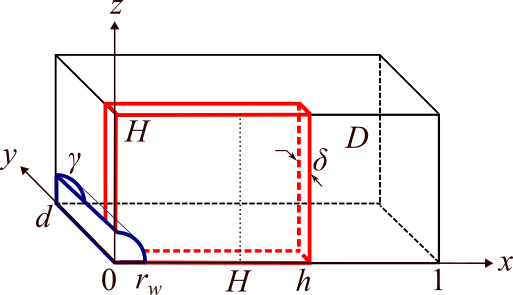
\includegraphics[width=0.7\linewidth]{images/schemes/kham_fract_inner_scheme.png}
% 	\caption{\label{fig:kham_inner_sector_scheme}Область решения задачи притока жидкости к горизонтальной скважине с трансверсальной трещиной ГРП}
% \end{figure}

% Будем различать два типа берегов трещин: внутренний~--~такой, справа или слева от которого есть соседние трещины; и внешний~--~такой, где справа или слева проходит граница области дренирования.

% Трехмерная задача для давления~$p$ в коллекторе~$D$ для однородного пласта с учетом плоской симметрии имеет вид~(\ref{eq:kham_main_p_res}) с граничными условиями
% \begin{equation}
% 	\displaystyle
% 	\begin{gathered}
% 		\left. p\right|_{\gamma} = 0; \quad p=1 \quad \text{при} \quad x = 1; \\
% 		\dfrac{\partial p}{\partial n} = 0 \quad \text{при} \quad x=0; \quad
% 		y = d; \quad y = 0, \quad x > h; \quad z = 0,1; \\
% 		p = p_f \quad \text{при} \quad y = 0, \quad x \leq h.
% 	\end{gathered}
% 	\label{eq:kham_inner_section_main_boundaries}
% \end{equation}

% Плоская задача для давления~$p_f$ в трещине ГРП при $y=0, \delta \longrightarrow 0$ и с учетом того, что плоскость~$y=0$ является плоскостью симметрии, имеет вид
% \begin{equation}
% 	\displaystyle
% 	\Delta p_f + \dfrac{1}{M} \left. \dfrac{\partial p}{\partial y} \right|_{y=\delta} = 0,
% 	\label{eq:kham_simple_main_pf}
% \end{equation}

% \begin{equation}
% 	\displaystyle
% 	\left. p_f \right|_{\gamma} = 0; \quad \dfrac{\partial p_f}{\partial n} = 0 \quad \text{при} \quad x=0, h.
% 	\label{eq:kham_simple_main_pf_boundaries}
% \end{equation}

% Нетрудно видеть, что для трещин бесконечной проводимости $M \longrightarrow \infty$ и
% (\ref{eq:kham_simple_main_pf}) превращается в уравнение $p_f = 0$, которое при граничных
% условиях (\ref{eq:kham_simple_main_pf_boundaries}) имеет тривиальное решение $p_f \equiv 0$.
% Напротив, для тонких плохопроводящих трещин $M \longrightarrow 0$, и уравнение (\ref{eq:kham_simple_main_pf}),
% предварительно умноженное на $M$ вырождается в равенство~$\partial p/\partial y = 0$, которое
% с учетом $p_f = p$ (\ref{eq:kham_simple_main_pf_boundaries}) приводит к рассмотренной в
% работе~\cite{lit:kham_mazo_uzku_2015} задаче о ГС без трещин ГРП.

% При конечных $M$ приближенное решение задачи можно получить, приняв два упрощения:
% \begin{enumerate}
% 	\item деление области внутри трещины на две подобласти: (а) $r_w \leq x < H$, (б) $H \leq x \leq h$;
% 	\item  аппроксимация второго члена уравнения (\ref{eq:kham_simple_main_pf}) при помощи выражения
% 	      \begin{equation}
% 		      \displaystyle
% 		      \dfrac{\partial p}{\partial y} \approx \dfrac{1}{d}\left(p_d - p_f\right),
% 		      \label{eq:kham_dpdy_approx}
% 	      \end{equation}
% 	      где~$p_d(x)$~--~давление в пласте в плоскости симметрии~$y=d$.
% 	      Если берег трещины внутренний, то $p_d$ вычисляется по формулам
% 	      распределения давления в  пласте, а если внешний, то возможны два варианта: трещина находится
% 	      от торца скважины на расстояние больше $d$, тогда можно считать ее как внутреннюю;
% 	      трещина находится непосредственно на торце скважины, тогда в формуле~(\ref{eq:kham_dpdy_approx})
% 	      следует положить $d = 1$, $p_d = 1$ (давление на контуре питания).
% \end{enumerate}

% \subsubsection{Внутренний берег трещины}

% \mysub{Подобласть (а) $r_w \leq x < H$}
% В трещине также воспользуемся допущением о том, что давление $p^f_{\Gamma}$ на
% границе $x=H$ близко к давлению на окружности $\Gamma_f=\left\{\left(x,z\right): \sqrt{x^2 + z^2} = H \right\}$. %chktex 21
% Тогда в подобласти, ограниченной окружностями $\gamma_f$ и $\Gamma_f$ и лучами $x=0$ и $z=0$
% фильтрация будет плоско-радиальной и описываться одномерной задачей с учетом (\ref{eq:kham_dpdy_approx})
% и (\ref{eq:kham_reservoir_press_inner_section_radial})
% \begin{equation}
% 	\displaystyle
% 	\begin{gathered}
% 		\dfrac{1}{r}\dfrac{d}{dr}\left(r\dfrac{d p_f}{dr}\right) - \dfrac{p_f}{Md} =
% 		- p^R_{\Gamma}\dfrac{1}{Md} \dfrac{\ln{\left(r/r_w\right)}}{\ln{\left(H/r_w\right)}}, \quad r_w < r < H;    \\[8pt]
% 		p_f = 0 \quad \text{при} \quad r = r_w; \quad p_f = p^f_{\Gamma} \quad \text{при} \quad r = H,
% 	\end{gathered}
% 	\label{eq:kham_fract_area_a_press_main}
% \end{equation}
% где $p^f_{\Gamma}$ — давление в трещине на границе $\Gamma_f$, $p^R_{\Gamma}$ — давление в
% пласте на границе $\Gamma$ в плоскости симметрии $y=d$.

% Уравнение~(\ref{eq:kham_fract_area_a_press_main}) линейное неоднородное дифференциальное уравнение второго порядка.
% Общее решение такого уравнения имеет вид
% \begin{equation}
% 	\displaystyle
% 	p_f(r) = p_f^h\left(r\right) + p_f^p\left(r\right),
% 	\label{eq:kham_kham_final_pf_ode_solution_view}
% \end{equation}
% где $p_f^h\left(x\right)$~--~решение однородного уравнения, а $p_f^p\left(x\right)$~--~неоднородного.
% Однородную часть уравнения~(\ref{eq:kham_fract_area_a_press_main}) можно записать в виде
% \begin{equation}
% 	\displaystyle
% 	\dfrac{1}{r}\dfrac{d}{dr}\left(r\dfrac{d p_f^h}{dr}\right) - \lambda^2 p_f^h = 0, \quad \lambda^2 = \dfrac{1}{Md} > 0
% 	\label{eq:kham_fract_inner_pf_part2_mono}
% \end{equation}
% Решение такого уравнения~(\ref{eq:kham_fract_inner_pf_part2_mono}) имеет вид
% \begin{equation}
% 	\displaystyle
% 	p_f^h\left(r\right) = A_a I_0\left(\lambda r\right) + B_a K_0\left(\lambda r\right),
% 	\label{eq:kham_fa2_press_uniform_solution_main}
% \end{equation}
% где $I_0, K_0$~--~модифицированные функции Бесселя первого и второго рода нулевого порядка соответственно,
% $A_a,B_a$~--~константы, определяемые из граничных условий~(\ref{eq:kham_fract_area_a_press_main}),
% после того как найдено решение неоднородной части уравнения.

% Рассмотрим неоднородное уравнение
% \begin{equation}
% 	\displaystyle
% 	\dfrac{1}{r}\dfrac{d}{dr}\left(r\dfrac{d p_f^p}{dr}\right) - \dfrac{p_f^p}{Md} = f\left(r\right), \quad
% 	f\left(r\right) = - \dfrac{p^R_{\Gamma}}{Md} \dfrac{\ln{\left(r/r_w\right)}}{\ln{\left(H/r_w\right)}}.
% 	\label{eq:kham_fa2_press_nonuniform_equation}
% \end{equation}
% Решение этого уравнения будем искать в виде
% \begin{equation}
% 	\displaystyle
% 	p_f^p\left(r\right) = C_a \ln\left(r/r_w\right).
% 	\label{eq:kham_fa2_nonunif_sol_form}
% \end{equation}
% Вид такого решения выбран исходя из вида правой части $f\left(r\right)$ уравнения~(\ref{eq:kham_fa2_press_nonuniform_equation}).
% Константу $C_a$ определим, подставив (\ref{eq:kham_fa2_nonunif_sol_form}) в~(\ref{eq:kham_fa2_press_nonuniform_equation})
% и приравняв коэффициенты при $\ln\left(r/r_w\right)$ в левой и правой частях уравнения. Отсюда получим, что
% \begin{equation}
% 	\displaystyle
% 	C_a = \dfrac{p^R_{\Gamma}}{\ln{\left(H/r_w\right)}}.
% 	\label{eq:kham_sol_nonunif_c_cf}
% \end{equation}

% Теперь, когда решение неоднородного уравнения найдено, коэффициенты $A_a, B_a$ определяются из решения системы
% линейных уравнений, полученных из граничных условий~(\ref{eq:kham_fract_area_a_press_main}), путем подставления
% в них (\ref{eq:kham_kham_final_pf_ode_solution_view})
% \begin{equation}
% 	\displaystyle
% 	\begin{gathered}
% 		A_a = - \dfrac{K_0 \left(\lambda r_w\right)}{D_a} \left(p^f_{\Gamma} - p^R_{\Gamma}\right), \quad
% 		B_a = \dfrac{I_0 \left(\lambda r_w\right)}{D_a} \left(p^f_{\Gamma} - p^R_{\Gamma}\right), \\[6pt]
% 		D_a = I_0 \left(\lambda r_w \right)K_0\left(\lambda H\right) - I_0\left(\lambda H\right) K_0\left(\lambda r_w\right)
% 	\end{gathered}
% 	\label{eq:kham_fa2_press_ab_sol}
% \end{equation}

% Тогда окончательно распределение давления в трещине в области (а) с учетом~(\ref{eq:kham_kham_final_pf_ode_solution_view}),
% (\ref{eq:kham_fa2_press_uniform_solution_main}), (\ref{eq:kham_fa2_nonunif_sol_form}), (\ref{eq:kham_sol_nonunif_c_cf}),
% (\ref{eq:kham_fa2_press_ab_sol}) будет определяться по формуле
% \begin{equation}
% 	\displaystyle
% 	\begin{gathered}
% 		p_f\left(r\right) = \left(p^f_{\Gamma} - p^R_{\Gamma}\right)
% 		\dfrac{E_a\left(r\right)}{D_a}
% 		+ p^R_{\Gamma} \dfrac{\ln\left(r/r_w\right)}{\ln{\left(H/r_w\right)}}, \quad
% 		r_w \leq r \leq H \\[6pt]
% 		E_a\left(r\right) = I_0\left(\lambda r_w\right)K_0\left(\lambda r\right) - K_0\left(\lambda r_w\right)I_0\left(\lambda r\right),
% 	\end{gathered}
% 	\label{eq:kham_final_sol_pf_radial}
% \end{equation}
% а расход $Q_a$ на грани $\Gamma_f$
% \begin{equation}
% 	\displaystyle
% 	\begin{gathered}
% 		Q_a = - \dfrac{\pi \theta \delta H}{2} \left. \dfrac{d p_f}{d r}\right|_{r=H} =
% 		\theta \left(    F_a \left(p^f_{\Gamma} - p^R_{\Gamma}\right) + G_a \right) , \\[8pt]
% 		F_a = \dfrac{\pi \delta H \lambda H_a\left(H\right)}{2D_a}, \quad
% 		G_a = -\dfrac{\pi \delta p^R_{\Gamma}}{2 \ln{\left(H/r_w\right)}},  \\[8pt]
% 		\dfrac{d p_f}{d r} = \left(p^f_{\Gamma} - p^R_{\Gamma}\right)
% 		\dfrac{-\lambda H_a\left(r\right)}{D_a} +
% 		\dfrac{p^R_{\Gamma}}{r \ln{\left(H/r_w\right)}}, \\[8pt]
% 		H_a\left(r\right) =
% 		I_0\left(\lambda r_w\right)K_1\left(\lambda r\right) +
% 		K_0\left(\lambda r_w\right)I_1\left(\lambda r\right),
% 	\end{gathered}
% 	\label{eq:kham_q_Gf}
% \end{equation}
% где $I_1, K_1$~--~модифицированные функции Бесселя первого порядка.

% \mysub{Подобласть (б) $H \leq x \leq h$}
% В подобласти (б) получим плоско-параллельную задачу и уравнение для давления $p_f$ будет иметь вид
% \begin{equation}
% 	\displaystyle
% 	\begin{gathered}
% 		\dfrac{d^2 p_f}{dx^2}-\dfrac{p_f}{Md}=-\dfrac{1}{Md}\left(p^R_{\Gamma} + (1 - p^R_{\Gamma})\dfrac{x - H}{1-H}\right), \quad H \leq x \leq h, \\
% 		p_f = p^f_{\Gamma}  \quad \text{при} \quad x = H; \quad \dfrac{\partial p_f}{\partial x} = 0 \quad \text{при} \quad x = h.
% 	\end{gathered}
% 	\label{eq:kham_approx_pf_part2}
% \end{equation}

% Уравнение~(\ref{eq:kham_approx_pf_part2}) линейное неоднородное дифференциальное уравнение второго порядка.
% Общее решение такого уравнения имеет вид~(\ref{eq:kham_kham_final_pf_ode_solution_view}).

% Однородная часть уравнения~(\ref{eq:kham_approx_pf_part2})
% \begin{equation}
% 	\displaystyle
% 	\dfrac{d^2 p_f^h}{dx^2}-\lambda^2 p_f^h = 0, \quad \text{где} \quad \lambda^2 = \dfrac{1}{Md} > 0
% 	\label{eq:kham_final_pf_part2_mono}
% \end{equation}
% Общее решение уравнения~(\ref{eq:kham_final_pf_part2_mono})
% \begin{equation}
% 	\displaystyle
% 	p_f^h = A_b e^{\lambda x} + B_b e^{-\lambda x},
% 	\label{eq:kham_final_pf_part2_mono_solution}
% \end{equation}
% где $A_b, B_b$~--~константы, которые определим из граничных условий~(\ref{eq:kham_approx_pf_part2}).

% В неоднородной части уравнения правая часть является линейной функцией вида
% \begin{equation}
% 	\displaystyle
% 	f\left(x\right)=\dfrac{1}{Md} \left(p^R_{\Gamma} + \dfrac{\left( 1-p^R_{\Gamma}\right)\left(x-H\right)}{\left(1-H\right)}\right).
% 	\label{eq:kham_fx}
% \end{equation}
% Частное решение неоднородного уравнения с правой частью вида~(\ref{eq:kham_fx}) ищется в виде линейной функции
% \begin{equation}
% 	\displaystyle
% 	p_f^p = C_b x + D_b.
% 	\label{eq:kham_partical_pf_part2}
% \end{equation}
% Коэффициенты $C_b, D_b$ получим, подставив~(\ref{eq:kham_partical_pf_part2}) в (\ref{eq:kham_approx_pf_part2})
% и приравняв соответствующие коэффициенты при $x$ и при свободном слагаемом
% \begin{equation}
% 	\displaystyle
% 	C_b = \dfrac{1-p^R_{\Gamma}}{1-H}, \quad
% 	D_b = p^R_{\Gamma} - C_b H.
% 	\label{eq:kham_cf_c_d}
% \end{equation}
% Коэффициенты $C_b, D_b$ определены в~(\ref{eq:kham_cf_c_d}), осталось определить коэффициенты $A_b, B_b$.
% Для этого, используя граничные условия из~(\ref{eq:kham_approx_pf_part2}), составим систему алгебраических уравнений
% \begin{equation}
% 	\displaystyle
% 	\begin{cases}
% 		A_b e^{\lambda H} + B_b e^{-\lambda H} + p^R_{\Gamma} = p^f_{\Gamma} \\
% 		A_b \lambda e^{\lambda h} - B_b \lambda e^{-\lambda h} + C_b = 0
% 	\end{cases}
% 	\label{eq:kham_slau_a_b}
% \end{equation}
% Решение системы~(\ref{eq:kham_slau_a_b})
% \begin{equation}
% 	\displaystyle
% 	A_b = \frac{\left(p^f_{\Gamma} - p^R_{\Gamma}\right) e^{- \lambda h} - \dfrac{C_b}{\lambda} e^{-\lambda H}}{\eta}, \quad
% 	B_b = \frac{\left(p^f_{\Gamma} - p^R_{\Gamma}\right) e^{\lambda h} + \dfrac{C_b}{\lambda} e^{\lambda H}}{\eta},
% 	\label{eq:kham_a_b_slau_solution}
% \end{equation}
% где $\eta = 2 \cosh{\left(\lambda \left(H-h\right)\right)}$.

% Подставив $A_b, \;B_b$ из~(\ref{eq:kham_a_b_slau_solution}) в~(\ref{eq:kham_final_pf_part2_mono_solution}),
% а $C_b, \;D_b$ из~(\ref{eq:kham_cf_c_d}) в~(\ref{eq:kham_partical_pf_part2}) и с
% учетом~(\ref{eq:kham_kham_final_pf_ode_solution_view}) получим аналитическое решение уравнения~(\ref{eq:kham_approx_pf_part2})
% \begin{equation}
% 	\displaystyle
% 	p_f(x) = A_b e^{\lambda x} + B_b e^{-\lambda x} + C_b x + D_b, \quad
% 	H \leq x \leq h.
% 	\label{eq:kham_final_press_sol_outer_area_fract}
% \end{equation}

% Расход через границу $x=H$ в трещине
% \begin{equation}
% 	\displaystyle
% 	Q_b = - \delta H \left. \frac{d p_f}{d x} \right|_{x=H}
% 	= - \delta H \left( A_b \lambda e^{\lambda H} - B_b \lambda e^{-\lambda H} + C_b \right),
% 	\label{eq:kham_fract_inner_Qb}
% \end{equation}

% \mysub{Полный приток к участку скважины с трещиной ГРП }
% Выражение для определения $p^f_{\Gamma}$ получим из условия $Q_a = Q_b$
% \begin{equation}
% 	\displaystyle
% 	\begin{gathered}
% 		p^f_{\Gamma} = p^R_{\Gamma} - \frac{\theta G_a +  J_b}{ \theta F_a + K_b}, \\
% 		J_b = \delta H\,C_b \left(1 - \tfrac{2}{\eta}\right),
% 		K_b =  \delta H\,\lambda \tanh\!\big(\lambda (H-h)\big). % chktex 21
% 	\end{gathered}
% 	\label{eq:kham_pfg_inner}
% \end{equation}

% Полный приток к четверти перфорированного участка ГС и к четверти внутреннего берега трещины ГРП
% с учетом (\ref{eq:kham_qw_inner}) и (\ref{eq:kham_q_Gf})
% \begin{equation}
% 	\displaystyle
% 	Q = Q_w + Q_f = \dfrac{\pi d p^R_{\Gamma}}{2 \ln{\left(H / r_w\right)}} + F_a \left(p^f_{\Gamma} - p^R_{\Gamma}\right) + G_a
% 	\label{eq:kham_fract_inner_q_total}
% \end{equation}

% Поправочный коэффициент $\theta$ здесь определяется как и раньше из условия равенства аналитического
% дебита $Q$~(\ref{eq:kham_fract_inner_q_total}) и полученного из численного решения аналогичной задачи $Q_{\text{num}}$
% \begin{equation}
% 	\displaystyle
% 	\theta =
% 	\frac{\big(Q_{\text{num}} - Q_w\big)\,K_b}
% 	{\,G_a K_b - F_a J_b - \big(Q_{\text{num}} - Q_w\big)F_a}.
% 	\label{eq:kham_theta_inner}
% \end{equation}

% \subsubsection{Внешний берег трещины}
% Внешний берег трещины может находится непосредственно на торце скважине или на некотором
% расстоянии $d_e$ от торца. Для внешнего берега в качестве пластового давления будем брать давление на контуре питания, который находится на расстоянии $1+d_e$ от торца скважины, как уже было упомянуто в пояснении к формуле~(\ref{eq:kham_dpdy_approx}).

% \mysub{Подобласть (а) $r_w \leq x < H$}
% Если в формуле~(\ref{eq:kham_dpdy_approx}) положить $p_d=1$, то уравнение для давления будет
% иметь следующий вид
% \begin{equation}
% 	\displaystyle
% 	\begin{gathered}
% 		\dfrac{1}{r}\dfrac{d}{dr}\left(r\dfrac{d p_f}{dr}\right) - \dfrac{p_f}{Md} = - \dfrac{1}{Md} , \quad r_w < r < H;    \\[8pt]
% 		p_f = 0 \quad \text{при} \quad r = r_w; \quad p_f = p^f_{\Gamma} \quad \text{при} \quad r = H,
% 	\end{gathered}
% 	\label{eq:kham_fract_outer_area_a_press_main}
% \end{equation}
% где $d = 1 + d_e$.

% Решение однородного уравнение будет аналогично~(\ref{eq:kham_fa2_press_uniform_solution_main}),
% а решение неоднородного $p_f^p = 1$.
% Тогда общее решение согласно~(\ref{eq:kham_kham_final_pf_ode_solution_view})
% \begin{equation}
% 	\displaystyle
% 	p_f(r) = A_a^E I_0\left(\lambda r\right) + B_a^E K_0\left(\lambda r\right) + 1
% 	\label{eq:kham_fract_outer_pa}
% \end{equation}
% с коэффициентами
% \begin{equation}
% 	\displaystyle
% 	A_a^E = - \dfrac{K_0 \left(\lambda H \right) + \left( p^f_{\Gamma} - 1 \right) K_0 \left( \lambda r_w \right)}{D_a}, \quad
% 	B_a^E = \dfrac{I_0 \left( \lambda H \right) + \left(p^f_{\Gamma} - 1 \right) I_0 \left(\lambda r_w \right) }{D_a}.
% 	\label{eq:kham_fract_outer_pa_cf_AB}
% \end{equation}

% Тогда окончательно распределение давления в трещине в области (а) будет описываться уравнением
% \begin{equation}
% 	\displaystyle
% 	\begin{gathered}
% 		p_f\left(r\right) = 1 + \dfrac{\left(p^f_{\Gamma}-1\right) E_a \left(r\right) + J_a^E\left(r\right)}{D_a}, \quad r_w \leq r < H, \\
% 		J_a^E(r) = I_0 \left(\lambda H \right) K_0 \left(\lambda r\right) - K_0 \left(\lambda H\right) I_0 \left(\lambda r \right).
% 	\end{gathered}
% 	\label{eq:kham_fract_outer_final_sol_pf_radial}
% \end{equation}

% Расход $Q_a$ на грани $\Gamma_f$
% \begin{equation}
% 	\displaystyle
% 	\begin{gathered}
% 		Q_a = - \dfrac{\pi \theta \delta H}{2} \left. \dfrac{d p_f}{d r} \right|_{r=H} =
% 		\theta \left(    F_a \left(p^f_{\Gamma} - 1\right) + G_a^E \right), \\[8pt]
% 		\dfrac{d p_f}{d r} =
% 		- \dfrac{\lambda}{D_a} \left( \left(p^f_{\Gamma} - 1 \right) H_a \left(r\right) + K_a^E \left(r \right) \right), \\[8pt]
% 		G_a^E = \dfrac{\pi \delta H \lambda K_a^E (H)}{2 D_a}, \quad
% 		K_a^E \left(r\right) = K_0\left(\lambda H\right)I_1\left(\lambda r\right) + I_0\left(\lambda H\right)K_1\left(\lambda r\right).
% 	\end{gathered}
% 	\label{eq:kham_fract_outer_qa}
% \end{equation}

% \mysub{Подобласть (б) $H \leq x \leq h$}
% В подобласти (б) получим плоско-параллельную задачу и уравнение для давления $p_f$ будет иметь вид
% \begin{equation}
% 	\displaystyle
% 	\begin{gathered}
% 		\dfrac{d^2 p_f}{dx^2}-\dfrac{p_f}{Md}=-\dfrac{1}{Md}, \quad H \leq x \leq h, \\[8pt]
% 		p_f = p^f_{\Gamma}  \quad \text{при} \quad x = H; \quad \dfrac{\partial p_f}{\partial x} = 0 \quad \text{при} \quad x = h.
% 	\end{gathered}
% 	\label{eq:kham_fract_out_pf_area_b}
% \end{equation}
% Решение однородной части аналогично~(\ref{eq:kham_final_pf_part2_mono_solution}), а реешение неоднородной части $p_f^p = 1$.

% Коэффициенты $A_b^E, B_b^E$ определяются из граничных условий~(\ref{eq:kham_fract_out_pf_area_b})
% \begin{equation}
% 	\displaystyle
% 	A_b^E = \frac{p_\Gamma^f - 1}{e^{\lambda H} + e^{2 \lambda h - \lambda H}}, \quad
% 	B_b^E = \frac{(p_\Gamma^f - 1) \, e^{2 \lambda h}}{e^{\lambda H} + e^{2 \lambda h - \lambda H}}.
% 	\label{eq:kham_fract_out_area_b_AB}
% \end{equation}

% Тогда получим уравнение для давления
% \begin{equation}
% 	\displaystyle
% 	p_f(x) = A_b^E e^{\lambda x} + B_b^E e^{-\lambda x} + 1, \quad
% 	H \leq x \leq h.
% 	\label{eq:kham_fract_out_final_press_area_b}
% \end{equation}

% Расход через границу $x=H$ в трещине
% \begin{equation}
% 	\displaystyle
% 	Q_b = - \delta H \left. \frac{d p_f}{d x} \right|_{x=H} = - \delta H \, \lambda \, (p_\Gamma^f - 1) \, C_b^E, \quad
% 	C_b^E = \frac{e^{\lambda H} - e^{2 \lambda h - \lambda H}}{e^{\lambda H} + e^{2 \lambda h - \lambda H}}.
% 	\label{eq:rate_x_H}
% \end{equation}

% \mysub{Полный приток к участку скважины с трещиной ГРП }
% Выражение для определения $p^f_{\Gamma}$ получим из условия $Q_a = Q_b$
% \begin{equation}
% 	\displaystyle
% 	\begin{gathered}
% 		p^f_{\Gamma} = 1 - \frac{\theta G_a^E }{\theta F_a + \delta H \lambda C_b^E}
% 	\end{gathered}
% 	\label{eq:kham_fract_out_pfg}
% \end{equation}

% Полный приток к четверти перфорированного участка ГС и к четверти внешнего берега трещины ГРП с
% учетом (\ref{eq:kham_qw_inner}) и (\ref{eq:kham_fract_outer_qa})
% \begin{equation}
% 	\displaystyle
% 	Q = Q_w + Q_f = \dfrac{\pi d_e p^R_{\Gamma}}{2 \ln{\left(H / r_w\right)}} +
% 	F_a \left(p^f_{\Gamma} - 1\right) + G_a^E.
% 	\label{eq:kham_q_total_inner}
% \end{equation}

% Поправочный коэффициент $\theta$ здесь определяется как и раньше из условия равенства аналитического
% дебита $Q$~(\ref{eq:kham_q_total_inner}) и полученного из численного решения аналогичной задачи $Q_{num}$
% \begin{equation}
% 	\displaystyle
% 	\theta = \dfrac{Q_\mathrm{num} - Q_w}{G_a^E - \dfrac{F_a}{\delta H \lambda C_b^E} \left( Q_\mathrm{num} - Q_w\right)}.
% 	\label{eq:kham_fract_out_theta}
% \end{equation}

% Библиография
% \cleardoublepage % Начинаем с новой страницы (для двусторонней печати)
\phantomsection % Для гиперссылок в PDF  chktex 1
\bibliographystyle{ugost2008}
%\bibliographystyle{ugost2008ls} % Стиль с сортировкой по упоминанию % или \bibliographystyle{ugost2008} % Алфавитная сортировка
\bibliography{references}
\addcontentsline{toc}{section}{Список литературы}

\end{document}
